%!TEX root = ../../prace.tex


\appendix
\chapwithtoc{Přílohy}

\renewcommand{\thesection}{\Alph{section}}

\section{Struktura souborů přílohy}


\section{Grafy k~dotazníku}
\label{sec:survey}


Níže je možné se podívat na grafy zpracované stránkou Google Forms. U~sloupcových grafů byla otázka zodpovězena na škále od 1 do 10. Krajní hodnoty, které byly v~dotazníku nabídnuty, jsou vepsány v~popisku obrázku.

\begin{figure}[!ht]\centering
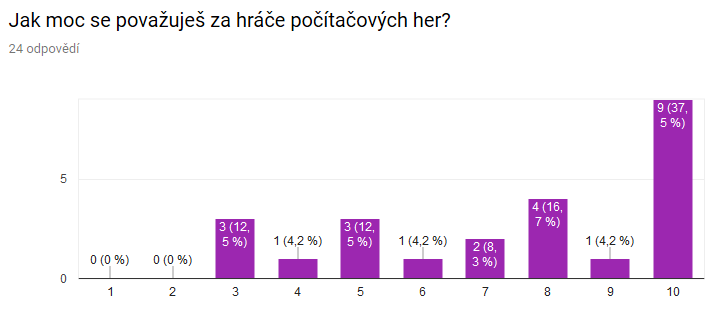
\includegraphics[ width=110mm]{../img/survey/q1}
\caption{Vůbec hry nehraji -- Hraji každý den}
\label{fig:q1}
\end{figure}
\FloatBarrier


\begin{figure}[!ht]\centering
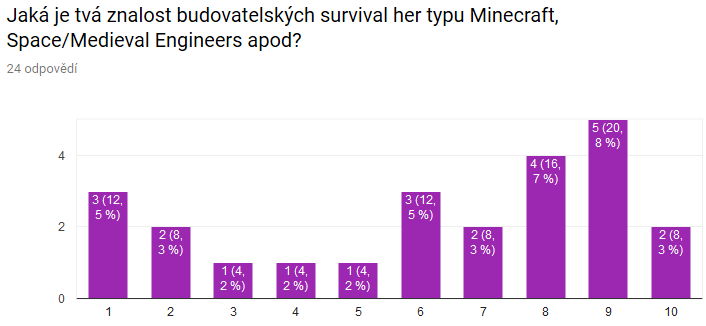
\includegraphics[ width=110mm]{../img/survey/q2}
\caption{Vůbec to neznám -- Znám je velice dobře}
\label{fig:q2}
\end{figure}
\FloatBarrier


\begin{figure}[!ht]\centering
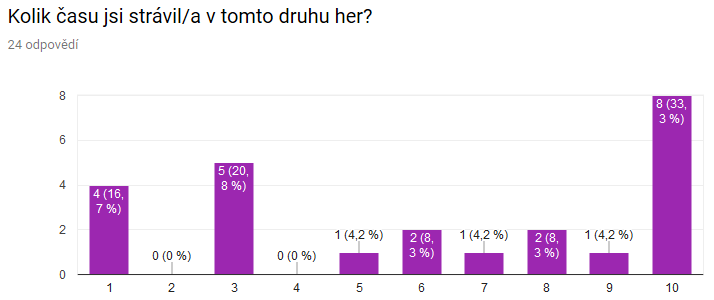
\includegraphics[ width=110mm]{../img/survey/q3}
\caption{Velice málo (max. 1 hodinu) -- Hodně (100 a~více hodin)}
\label{fig:q3}
\end{figure}
\FloatBarrier


\begin{figure}[!ht]\centering
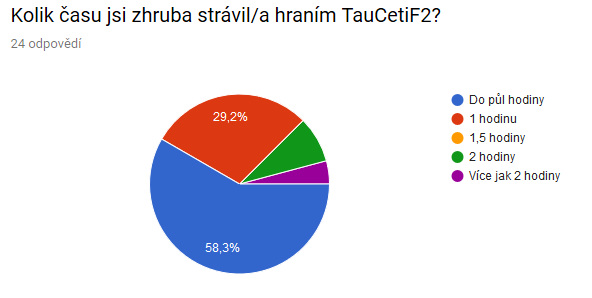
\includegraphics[ width=110mm]{../img/survey/q4}
\caption{Otázka 4}
\label{fig:q4}
\end{figure}
\FloatBarrier


\begin{figure}[!ht]\centering
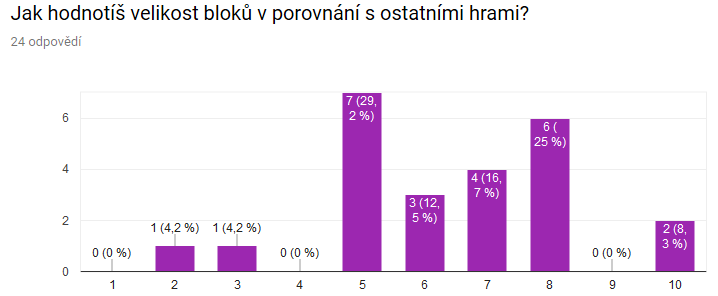
\includegraphics[ width=110mm]{../img/survey/q5}
\caption{Příliš malé -- Dostatečně velké}
\label{fig:q5}
\end{figure}
\FloatBarrier


\begin{figure}[!ht]\centering
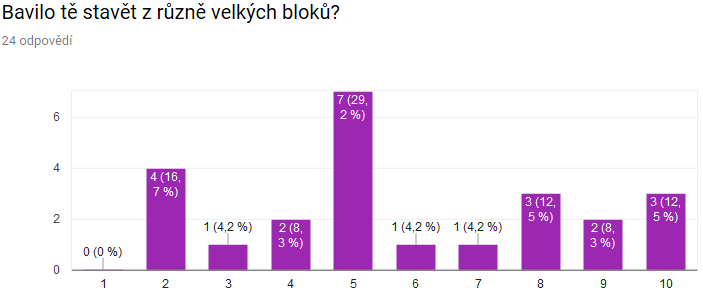
\includegraphics[ width=110mm]{../img/survey/q6}
\caption{Stavění bylo oproti jiným hrám nepříjemné -- Stavění mě oproti jiným hrám opravdu bavilo}
\label{fig:q6}
\end{figure}
\FloatBarrier


\begin{figure}[!ht]\centering
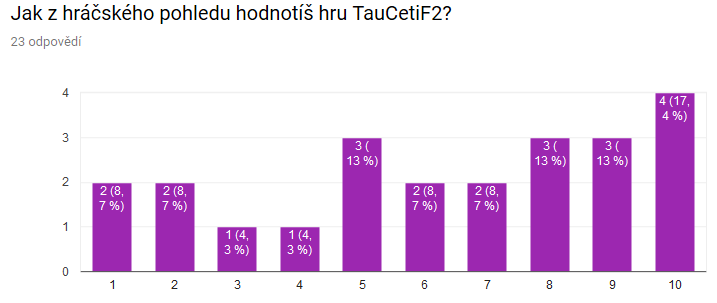
\includegraphics[ width=110mm]{../img/survey/q7}
\caption{Velice nepovedená, nikdy se k~ní nevrátím -- Zdařilá, rád/a bych si v~budoucnu dokončenou hru zahrál/a}
\label{fig:q7}
\end{figure}
\FloatBarrier